
\begin{myframe}{FFT: Derivation (1) }
\centering
\begin{align*}
F_N (k)&= \dft = \sumnn x(2n) \wn{k (2n)} + \sumnn x(2n+1) \wn{k (2n+1)} \\
&= \sumnn x(2n) \wn{k 2 n} + \wn{k} \sumnn x(2n+1) \wn{k(2n)} \\
&= \sumnn x(2n) \wnn{kn} + \wn{k} \sumnn x(2n+1) \wnn{kn} \\
&= \fnneven (k) + \wn{k} \fnnodd (k) \qquad k=0,\dots,(N-1)
\end{align*}

\begin{block}{}
\centering
$\wn{k}$ are called \textit{twiddle factors}
\end{block}

\end{myframe}

\begin{myframe}{FFT: Derivation (2)}
\centering

\begin{block}{}
\centering
¿Value of $\fnneven(k)$ and $\fnnodd(k)$ if $k \geq N/2$?
\end{block}

Define $N_1=\{ 0,\dots,N/2-1 \}$ and $N_2=\{ N/2,\dots,N-1 \}$
%\small
\begin{align*}
\fn (k)&= \fnneven (k) + \wn{k} \fnnodd (k)\\
&= \begin{cases}
\fnneven (k) + \wn{k} \fnnodd (k) &\mbox{if } k \in N_1 \\
\fnneven (k) + \wn{k} \fnnodd (k) & \mbox{if } k \in N_2 \\
\end{cases}
\\  \text{If } k\geq N/2 &\rightarrow k=N/2+k'
\\ &= \begin{cases}
\fnneven (k) + \wn{k} \fnnodd (k) &\mbox{if } k \in N_1 \\
\fnneven (N/2+k') + \wn{N/2+k'} \fnnodd (N/2+k') & \mbox{if } k' \in N_1
\end{cases}
\\ &= \begin{cases}
\fnneven (k) + \wn{k} \fnnodd (k) & \mbox{if } k \in N_1 \\
\fnneven (k') - \wn{k'} \fnnodd (k') & \mbox{if } k' \in N_1
\end{cases}
\end{align*}

\end{myframe}

\begin{myframe}{FFT: Divide and conquer}
\centering
\begin{block}{Calculating $\fn(k)$ for all $k$}
\begin{enumerate}
\item Split $x(n)$ into $x_{odd}(n)$ and $x_{even}(n)$.
\item Calculate $\fnneven(k)$ and $\fnnodd(k)$ for all $k$
\item Calculate $\fn(k)$ for all $k$ as:
\begin{equation}
\fn (k) = \begin{cases}
\fnneven (k) + \wn{k} \fnnodd (k) & \mbox{if } k \in N_1 \\
\fnneven (k') - \wn{k'} \fnnodd (k') & \mbox{if } k' \in N_1, \; k=N/2+k'
\end{cases}
\end{equation}

\end{enumerate}
\end{block}
\end{myframe}

\begin{myframe}{FFT: Recursion splits}
\centering
\scalebox{0.75}{
    
\newcommand{\gridthing}[3]{ 




\pgfmathtruncatemacro\fend{#1/2-1} 

\foreach \s in {0,...,\fend}{
    \pgfmathtruncatemacro\xpos{#2-#1/2+\s*2} 
    \filldraw[fill=white] (\xpos,#3-1) rectangle (\xpos+1,#3);
}

\foreach \s in {0,...,\fend}{
    \pgfmathtruncatemacro\xpos{#2-#1/2+\s*2} 
    \filldraw[fill=gray!10] (\xpos+1,#3-1) rectangle (\xpos+2,#3);
}

}

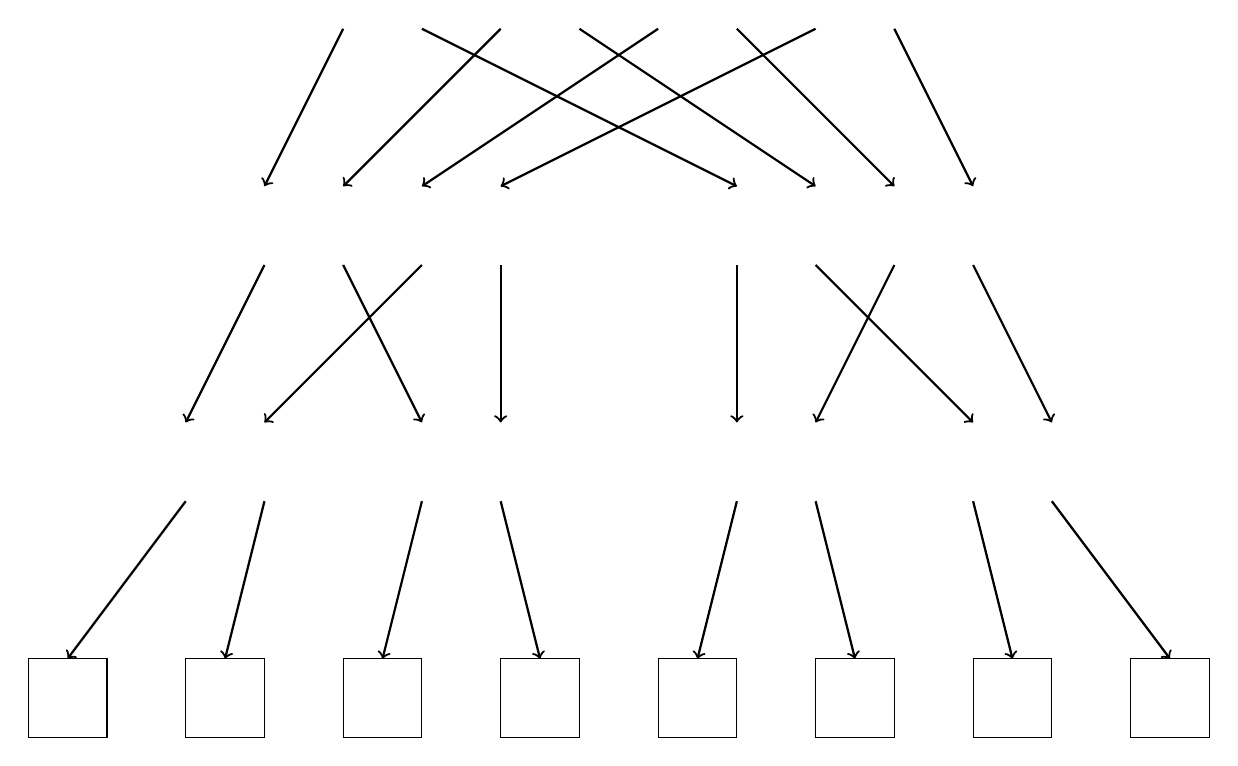
\begin{tikzpicture}[level/.style={sibling distance=60mm/#1}]

\gridthing{8}{0}{9}

\draw[thick,->] (-3.5,8) -- (-4.5,6);
\draw[thick,->] (-1.5,8) -- (-3.5,6);
\draw[thick,->] (0.5,8) -- (-2.5,6);
\draw[thick,->] (2.5,8) -- (-1.5,6);

\draw[thick,->] (3.5,8) -- (4.5,6);
\draw[thick,->] (1.5,8) -- (3.5,6);
\draw[thick,->] (-0.5,8) -- (2.5,6);
\draw[thick,->] (-2.5,8) -- (1.5,6);

\gridthing{4}{-3}{6}
\gridthing{4}{3}{6}

\draw[thick,->] (-4.5,5) -- (-5.5,3);
\draw[thick,->] (-3.5,5) -- (-2.5,3);
\draw[thick,->] (-2.5,5) -- (-4.5,3);
\draw[thick,->] (-1.5,5) -- (-1.5,3);

\draw[thick,->] (4.5,5) -- (5.5,3);
\draw[thick,->] (3.5,5) -- (2.5,3);
\draw[thick,->] (2.5,5) -- (4.5,3);
\draw[thick,->] (1.5,5) -- (1.5,3);

\gridthing{2}{-5}{3}
\gridthing{2}{-2}{3}
\gridthing{2}{2}{3}
\gridthing{2}{5}{3}

\draw[thick,->] (-5.5,2) -- (-7,0);
\draw[thick,->] (-4.5,2) -- (-5,0);
\draw[thick,->] (-2.5,2) -- (-3,0);
\draw[thick,->] (-1.5,2) -- (-1,0);

\draw[thick,->] (5.5,2) -- (7,0);
\draw[thick,->] (4.5,2) -- (5,0);
\draw[thick,->] (2.5,2) -- (3,0);
\draw[thick,->] (1.5,2) -- (1,0);

\foreach \l in {0,...,7}{
    \filldraw[fill=white] (\l*2-7.5,0) rectangle (\l*2-6.5,-1);
}

%\foreach \l in {8,4,2}{
%    \pgfmathtruncatemacro\basexpos{\l} 
%    \pgfmathtruncatemacro\ypos{ln(\l)/ln(2)} 
%
%    \pgfmathtruncatemacro\items{4-\ypos} 
%    \foreach \b in {1,...,\items}{
%        \pgfmathtruncatemacro\xposs{\basexpos*(\b-1)} 
%        \gridthing{\basexpos}{\xposs}{\ypos*3}
%     }
%}



%\gridthing{4}{1}{3}


\end{tikzpicture}

} 
\end{myframe}

\begin{myframe}{FFT: Recursion tree}
\centering
\scalebox{0.85}{
    
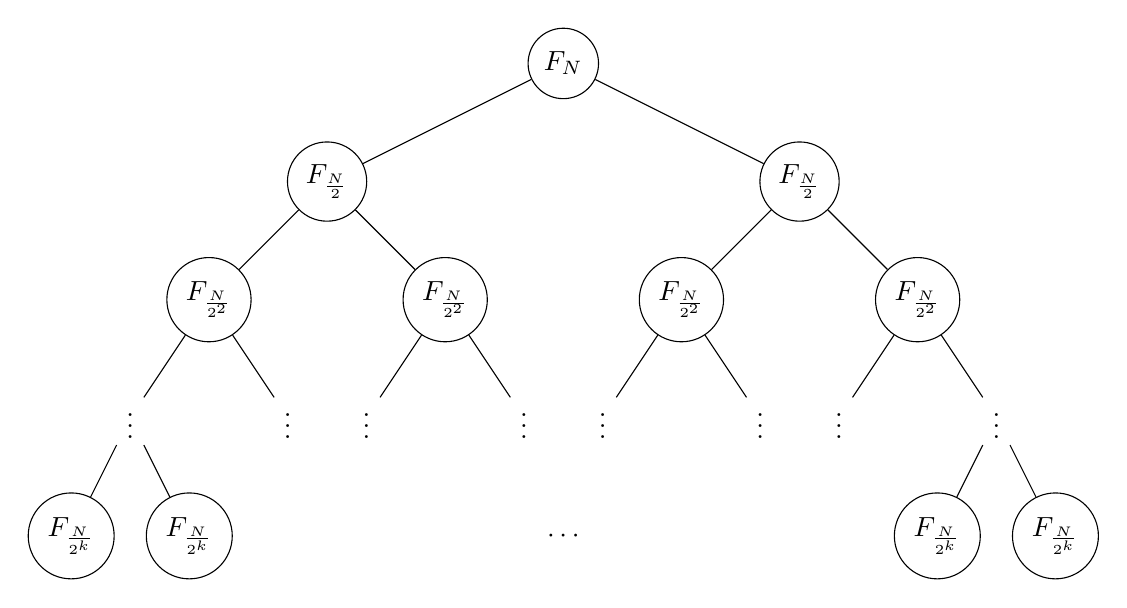
\begin{tikzpicture}[level/.style={sibling distance=60mm/#1}]

\node [circle,draw] (z){$F_N$}
  child {node [circle,draw] (a) {$F_{\frac{N}{2}}$}
    child {node [circle,draw] (b) {$F_{\frac{N}{2^2}}$}
      child {node {$\vdots$}
        child {node [circle,draw] (d) {$F_{\frac{N}{2^k}}$}}
        child {node [circle,draw] (e) {$F_{\frac{N}{2^k}}$}}
      } 
      child {node {$\vdots$}}
    }
    child {node [circle,draw] (g) {$F_{\frac{N}{2^2}}$}
      child {node {$\vdots$}}
      child {node {$\vdots$}}
    }
  }
  child {node [circle,draw] (j) {$F_{\frac{N}{2}}$}
    child {node [circle,draw] (k) {$F_{\frac{N}{2^2}}$}
      child {node {$\vdots$}}
      child {node {$\vdots$}}
    }
    child {node [circle,draw] (l) {$F_{\frac{N}{2^2}}$}
        child {node {$\vdots$}}
        child {node (c){$\vdots$}
          child {node [circle,draw] (o) {$F_{\frac{N}{2^k}}$}}
          child {node [circle,draw] (p) {$F_{\frac{N}{2^k}}$}
          }
        }
    }
  }    
;
\path (o) -- (e) node (x) [midway] {$\cdots$};

\end{tikzpicture}

} 
\end{myframe}

\begin{myframe}{FFT: Implementation}
\centering
\lstinputlisting[basicstyle=\small\ttfamily]{code/facuft.m}
\end{myframe}

\begin{myframe}{FFT: Time complexity}
\centering
\lstinputlisting[basicstyle=\small\ttfamily]{code/facuft_time.m}
\end{myframe}

\begin{myframe}{FFT: Solving recurrence}
\centering

\only<1>{
\begin{block}{}
\begin{equation*}
T(n)= 
\begin{cases}
    D & \mbox{if} \; n=1 \\
    2T(\frac{n}{2})+Cn & \mbox{if} \; n > 1
\end{cases}
\end{equation*}
\end{block}
}

\only<2->{
\begin{block}{}
\begin{equation*}
T(n)= 
\begin{cases}
    1 & \mbox{if} \; n=1 \\
    2T(\frac{n}{2})+n & \mbox{if} \; n > 1
\end{cases}
\end{equation*}
\end{block}
}

\only<3>{
\begin{align*}
T(n)&= 2T(\frac{n}{2})+n = 2 (2T(\frac{n}{2^2})+\frac{n}{2})+n = 2^2 T(\frac{n}{2^2})+2\frac{n}{2}+n \\
&= 2^2 T(\frac{n}{2^2})+2n = \dots = 2^k T(\frac{n}{2^k})+kn \\
\mbox{If } \frac{n}{2^k}=1 &\rightarrow k = \log_2(n): \\
T(n)&= 2^{\log_2(n)} T(1) + \log_2(n) n = n+n \log_2(n) \in O(n \log(n))
\end{align*}
}

\end{myframe}

\begin{myframe}{FFT: Time complexity with recursion tree}
\centering
\scalebox{0.71}{
    
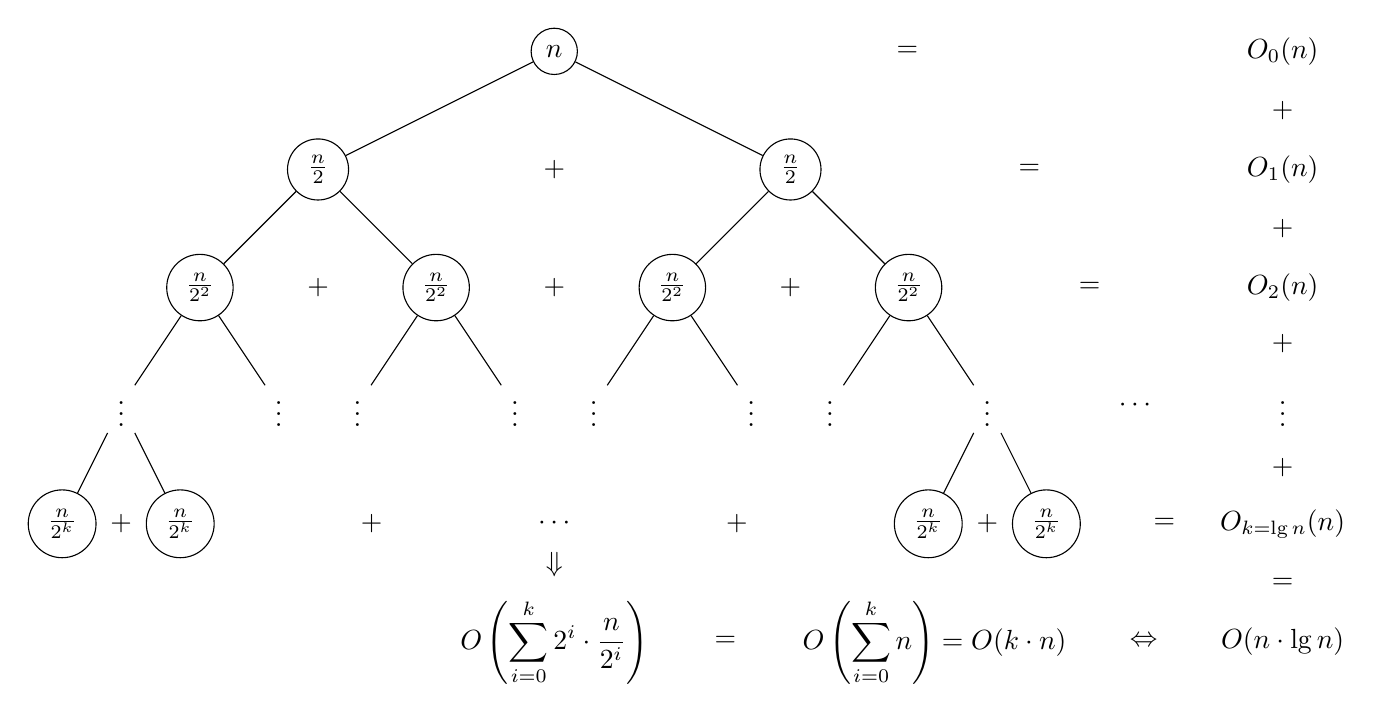
\begin{tikzpicture}[level/.style={sibling distance=60mm/#1}]
\node [circle,draw] (z){$n$}
  child {node [circle,draw] (a) {$\frac{n}{2}$}
    child {node [circle,draw] (b) {$\frac{n}{2^2}$}
      child {node {$\vdots$}
        child {node [circle,draw] (d) {$\frac{n}{2^k}$}}
        child {node [circle,draw] (e) {$\frac{n}{2^k}$}}
      } 
      child {node {$\vdots$}}
    }
    child {node [circle,draw] (g) {$\frac{n}{2^2}$}
      child {node {$\vdots$}}
      child {node {$\vdots$}}
    }
  }
  child {node [circle,draw] (j) {$\frac{n}{2}$}
    child {node [circle,draw] (k) {$\frac{n}{2^2}$}
      child {node {$\vdots$}}
      child {node {$\vdots$}}
    }
  child {node [circle,draw] (l) {$\frac{n}{2^2}$}
    child {node {$\vdots$}}
    child {node (c){$\vdots$}
      child {node [circle,draw] (o) {$\frac{n}{2^k}$}}
      child {node [circle,draw] (p) {$\frac{n}{2^k}$}
        child [grow=right] {node (q) {$=$} edge from parent[draw=none]
          child [grow=right] {node (q) {$O_{k = \lg n}(n)$} edge from parent[draw=none]
            child [grow=up] {node (r) {$\vdots$} edge from parent[draw=none]
              child [grow=up] {node (s) {$O_2(n)$} edge from parent[draw=none]
                child [grow=up] {node (t) {$O_1(n)$} edge from parent[draw=none]
                  child [grow=up] {node (u) {$O_0(n)$} edge from parent[draw=none]}
                }
              }
            }
            child [grow=down] {node (v) {$O(n \cdot \lg n)$}edge from parent[draw=none]}
          }
        }
      }
    }
  }
};
\path (a) -- (j) node [midway] {+};
\path (b) -- (g) node [midway] {+};
\path (k) -- (l) node [midway] {+};
\path (k) -- (g) node [midway] {+};
\path (d) -- (e) node [midway] {+};
\path (o) -- (p) node [midway] {+};
\path (o) -- (e) node (x) [midway] {$\cdots$}
  child [grow=down] {
    node (y) {$O\left(\displaystyle\sum_{i = 0}^k 2^i \cdot \frac{n}{2^i}\right)$}
    edge from parent[draw=none]
  };
\path (q) -- (r) node [midway] {+};
\path (s) -- (r) node [midway] {+};
\path (s) -- (t) node [midway] {+};
\path (s) -- (l) node [midway] {=};
\path (t) -- (u) node [midway] {+};
\path (z) -- (u) node [midway] {=};
\path (j) -- (t) node [midway] {=};
\path (y) -- (x) node [midway] {$\Downarrow$};
\path (v) -- (y)
  node (w) [midway] {$O\left(\displaystyle\sum_{i = 0}^k n\right) = O(k \cdot n)$};
\path (q) -- (v) node [midway] {=};
\path (e) -- (x) node [midway] {+};
\path (o) -- (x) node [midway] {+};
\path (y) -- (w) node [midway] {$=$};
\path (v) -- (w) node [midway] {$\Leftrightarrow$};
\path (r) -- (c) node [midway] {$\cdots$};
\end{tikzpicture}

} 
\end{myframe}

\begin{myframe}{FFT: Output}
\centering
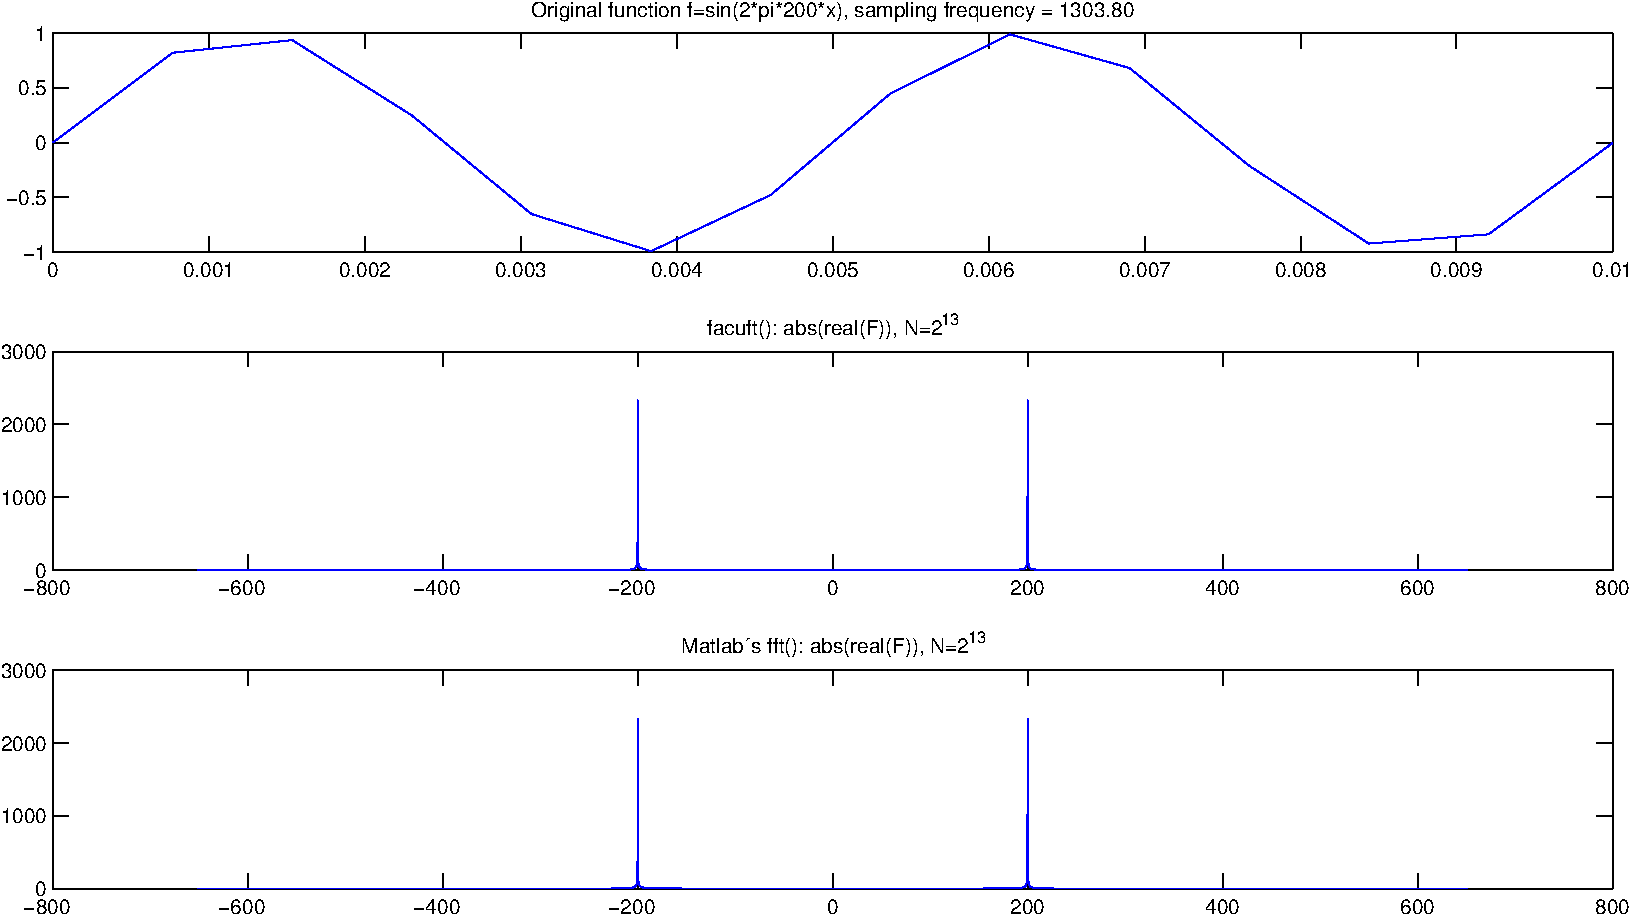
\includegraphics[height=200pt]{img/facuft}
\end{myframe}

\begin{myframe}{FFT: Empirical running time}
\centering
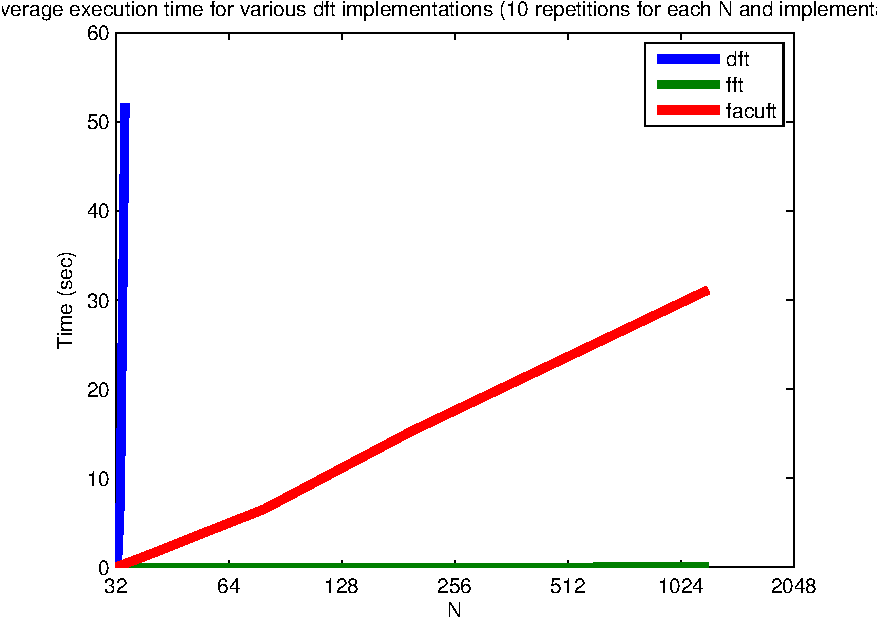
\includegraphics[height=200pt]{img/running_time}
\end{myframe}

\begin{myframe}{FFT: Implementation improvements}
\centering
\begin{itemize}
\item Recursion kills performance $\rightarrow$ bigger base cases
\item In every recursion call, split the input $x$ into $K$ subarrays instead of 2 (tree depth $= \log_K(n)$, \textit{fatter} trees) $\rightarrow$ Radix-m algorithms.
\item Recursion kills performance $\rightarrow$ iterative implementation
\item Calculate in-place (ie, no temporary arrays)
\item Avoid pure matlab (matlab's \texttt{fft} is written in C)
\item DFT's lower bound not known, but many results pointing to $DFT \in \Omega(n \log(n))$
\end{itemize}
\end{myframe}

\begin{myframe}{FFT: Bigger base case}
\centering
\lstinputlisting[basicstyle=\small\ttfamily]{code/facuft_basecase.m}
\end{myframe}

\begin{myframe}{FFT: Empirical running time}
\centering
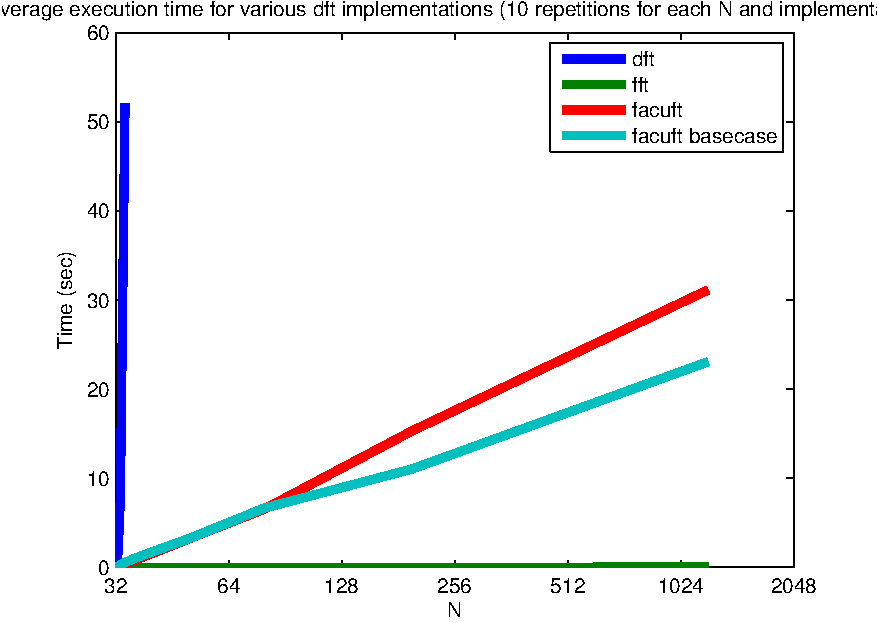
\includegraphics[height=200pt]{img/running_time_basecase}
\end{myframe}